\begin{figure}[htbp]
\centering
\begin{tikzpicture}[x=1cm,y=1cm]
\node[anchor=south west,inner sep=0] at (0,0) {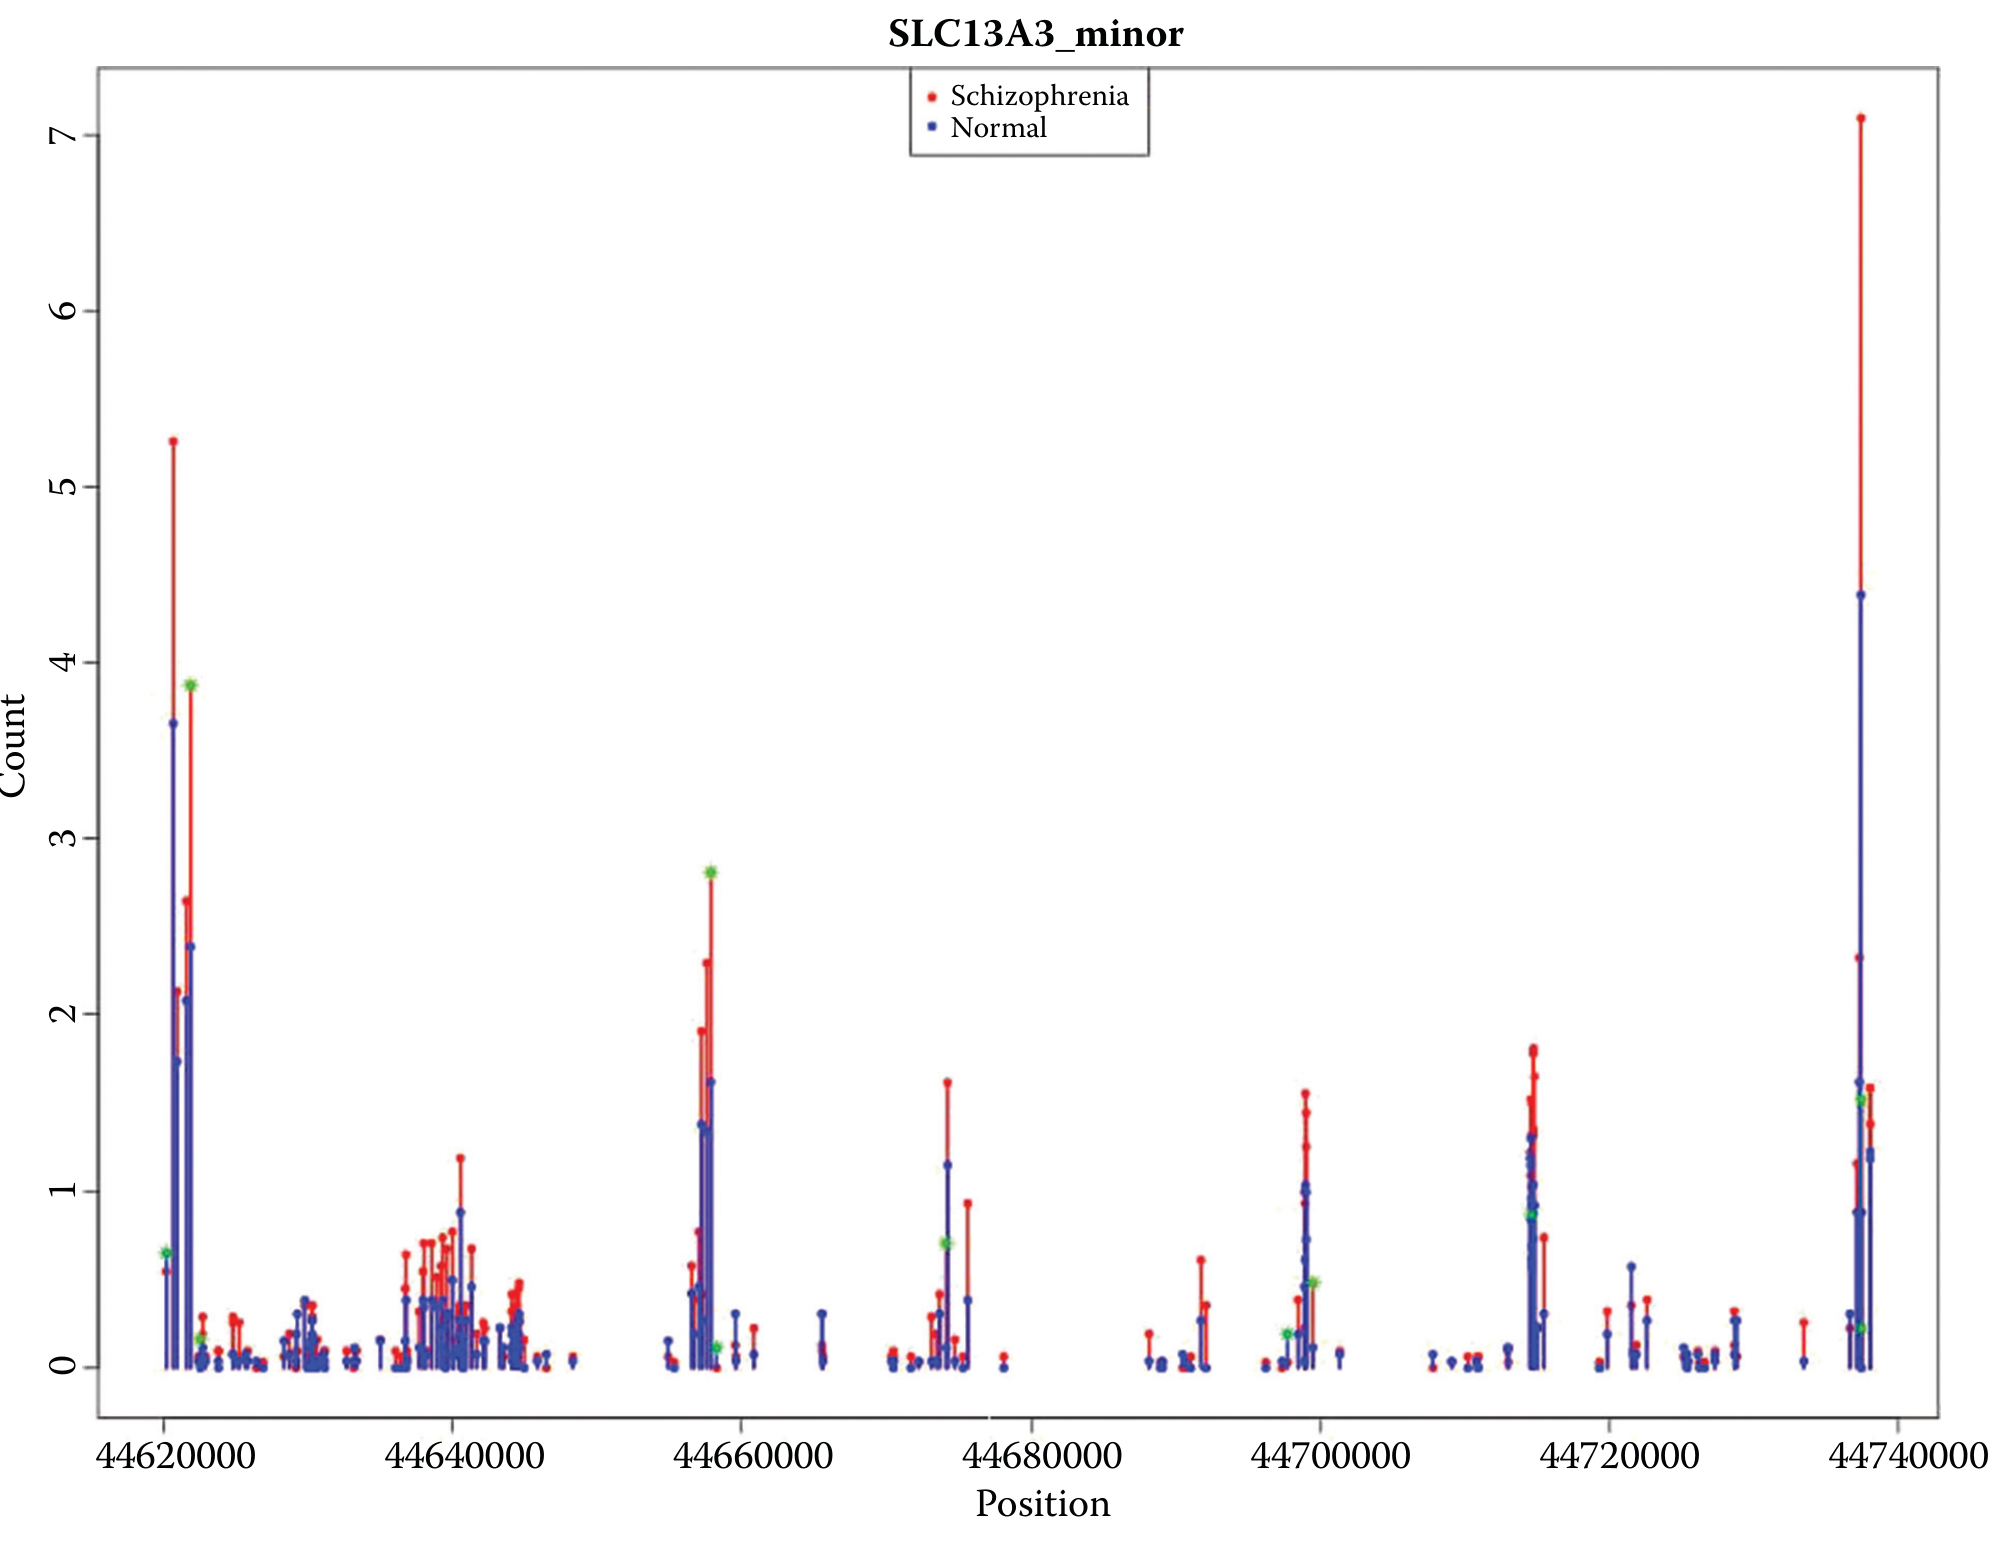
\includegraphics[width=12.0cm]{figures/ch04a_fig15_data.png}};
\fill[white] (5.6775,8.5683) rectangle (6.8042,8.7983);
\node[inner sep=0pt,fill=white,rotate=0,font=\fontsize{6}{8}\selectfont] at (6.2409,8.6833) {精神分裂症};
\fill[white] (5.3035,8.9120) rectangle (7.1288,9.2020);
\node[inner sep=0pt,fill=white,rotate=0,font=\fontsize{8}{8}\selectfont] at (6.2162,9.0570) {SLC13A3：次要等位基因};
\fill[white] (5.6775,8.3801) rectangle (6.3104,8.6101);
\node[inner sep=0pt,fill=white,rotate=0,font=\fontsize{6}{8}\selectfont] at (5.9939,8.4951) {正常};
\fill[white] (-0.1235,4.4508) rectangle (0.3515,5.1332);
\node[inner sep=0pt,fill=white,rotate=90,font=\fontsize{8}{8}\selectfont] at (0.0465,4.7920) {计数};
\fill[white] (5.8239,0.0903) rectangle (6.6934,0.3803);
\node[inner sep=0pt,fill=white,rotate=0,font=\fontsize{8}{8}\selectfont] at (6.2586,0.2353) {位置};
\end{tikzpicture}
\origfig{15}{基因 SLC13A3 次要等位基因的差异表达。}
\label{fig:ch04a-15}
\end{figure}
